\documentclass{article}
\usepackage{graphicx} % Required for inserting images
\usepackage{pgfplots} % For making the axes
\usepackage{geometry} % For plotting functions
\usepackage{amsmath, amsthm, amssymb, amsfonts}
\usepackage{thmtools}
\usepackage{setspace}
\usepackage{float}
\usepackage{hyperref}
\usepackage[utf8]{inputenc}
\usepackage[english]{babel}
\usepackage{framed}
\usepackage[dvipsnames]{xcolor}
\usepackage{tcolorbox}

\colorlet{LightGray}{White!90!Periwinkle}
\colorlet{LightOrange}{Orange!15}
\colorlet{LightGreen}{Green!15}

\declaretheoremstyle[name=Theorem]{thmsty}
\declaretheorem[style=thmsty,numberwithin=section]{theorem}
\tcolorboxenvironment{theorem}{colback=LightGray}

\declaretheoremstyle[name=Proposition,]{prosty}
\declaretheorem[style=prosty,numberlike=theorem]{proposition}
\tcolorboxenvironment{proposition}{colback=LightOrange}

\declaretheoremstyle[name=Principle,]{prcpsty}
\declaretheorem[style=prcpsty,numberlike=theorem]{principle}
\tcolorboxenvironment{principle}{colback=LightGreen}

\title{Unit 1 - Vectors and spaces}
\author{Francisco Dall' Oglio Scorsato}
\date{May 12th 2024}
\pgfplotsset{compat=1.18}

\begin{document}

\maketitle

\section{Lesson 1: Vectors}

\subsection{Vector intro for linear algebra}

A vector has magnitude and direction. If someone is going at "$5km/h$", that isn't a vector. 
However, if someone is going at "$5km/h$ east", since there is magnitude and direction, that is a vector.\\
\\
A vector will have a $x$ and $y$ component, and can be described like this:
\[\vec{v}=(x,y)\]
For the sake of this course, the matrix representation will be used more commonly. That is:
\[\vec{v}=
    \begin{bmatrix}
     x\\
     y
    \end{bmatrix}\]
A vector $\vec{v}=(3,4)$ could be drawn the following way:\\
\begin{center}
    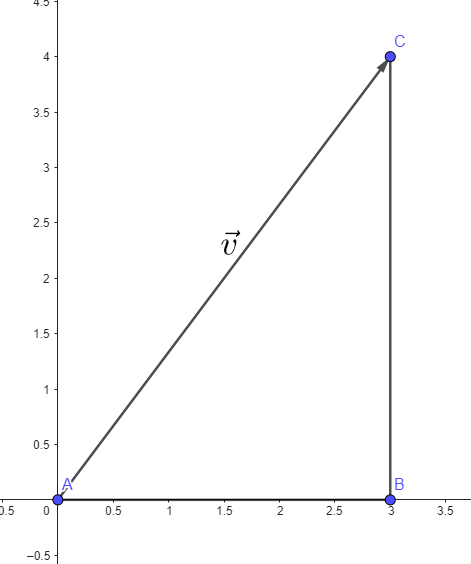
\includegraphics[scale=0.5]{image 1.png}
\end{center}
Notice that it's magnitude, per the Pythagorean Theorem, will be \(5\). 

\subsection{Real coordinate spaces}

We can represent the 2-dimensional real coordinate space (a.k.a the cartesian plane) as \(\mathbb{R}^2\).
That will be all possible real-valued "2-tuples". In our case, these "2-tuples" are the vectors that have two values.
All possible combinations of \(x\) and \(y\), both real, make \(\mathbb{R}^2\).\\
\par \(\mathbb{R}^3\) would be the $3D$ real coordinate space, with all real-valued 3-tuples. Or, 3 dimensional vectors.
In general, \(\mathbb{R}^n\) represents an n-dimensional real coordinate space with n-tuples.

\subsection{Adding vectors algebraically \& graphically}

Let \(\vec{a}=\begin{bmatrix}
    6\\
    -2
\end{bmatrix}\)
and \(\vec{b}=\begin{bmatrix}
    -4\\
    4
\end{bmatrix}\)

\[\vec{a}+\vec{b}=\begin{bmatrix}
    6 + (-4)\\
    -2 + 4
\end{bmatrix}= \begin{bmatrix}
    2\\
    2
\end{bmatrix}\]

Graphically, this is:
\begin{center}
    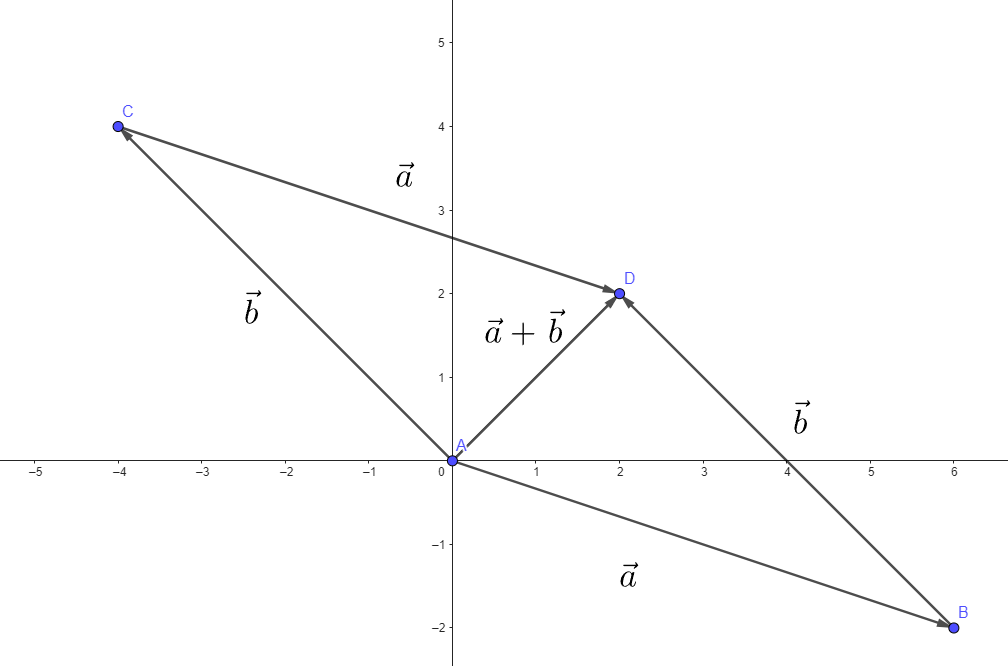
\includegraphics[scale=0.5]{image 2.png}
\end{center}

\begin{theorem}
    The sum of two vectors $\vec{a}$ and $\vec{b}$ such that $\vec{a}=(x_1,y_1)$ and $\vec{b}=(x_2,y_2)$ is $\vec{a}+\vec{b}=(x_1+x_2,y_1+y_2).$
\end{theorem}

\end{document}